\newif\ifjapanese
\japanesetrue  % 論文全体を日本語で書く(英語で書くならコメントアウト)
\ifjapanese
  %\documentclass[a4j,twoside,openright,11pt]{jreport} % 両面印刷の場合。余白を綴じ側に作って右起こし。
  \documentclass[a4j,11pt]{jreport}                  % 片面印刷の場合。
  \renewcommand{\bibname}{参考文献}
  \newcommand{\acknowledgmentname}{謝辞}
\else
  \documentclass[a4paper,11pt]{report}
  \newcommand{\acknowledgmentname}{Acknowledgment}
\fi
\usepackage[dvipdfmx]{graphicx}
\usepackage{thesis}
\usepackage{ascmac}
\usepackage{graphicx}
\usepackage{multirow}
\usepackage{url}
\usepackage{latexsym}
\usepackage{here}
\usepackage{listings,jlisting}

\lstset{%
  language={C},
  basicstyle={\small\ttfamily\footnotesize},%
  breaklines=true,%
  identifierstyle={\small},%
  commentstyle={\small\itshape},%
  keywordstyle={\small\bfseries},%
  ndkeywordstyle={\small},%
  stringstyle={\small\ttfamily},
  frame={tb},
  breaklines=true,
  columns=[l]{fullflexible},%
  numbers=left,%
  xrightmargin=0zw,%
  xleftmargin=3zw,%
  numberstyle={\scriptsize},%
  stepnumber=1,
  numbersep=1zw,%
  lineskip=-0.5ex%
}
\bibliographystyle{jwiss}

%\bindermode  % バインダー用余白設定

% 日本語情報(必要なら)
\jclass  {卒業論文}                             % 論文種別
\jtitle    {Gyaon \\ 音声活用の幅を広げる録音/共有システム}    % タイトル。改行する場合は\\を入れる
\juniv    {慶應義塾大学}                  % 大学名
\jfaculty  {環境情報学部}               % 学部、学科
\jauthor  {佐竹 紘明}                       % 著者
\jhyear  {28}                                   % 平成○年度
\jsyear  {2016}                                 % 西暦○年度
\jkeyword  {音声, 録音, インターフェース}     % 論文のキーワード
\jproject{増井俊之研究会} %プロジェクト名
\jdate{2017年1月}

\begin{document}

\ifjapanese
  \jmaketitle    % 表紙(日本語)
\else
  \emaketitle    % 表紙(英語)
\fi

% 日本語のアブストラクト
\begin{jabstract}
  TBD
\end{jabstract}
  % アブストラクト。要独自コマンド、include先参照のこと

\tableofcontents  % 目次
\listoffigures    % 図目次
% \listoftables    % 表目次

\pagenumbering{arabic}

\chapter{序論}
\label{chap:introduction}

本章では,本研究の背景と目的,および本論文の構成について述べる.

\newpage

\section{背景}

録音が可能な各種の小型レコーダ装置は古くから販売されており,またスマートフォンでは様々な録音アプリケーションを利用できる.
これらは音楽に携わる人やインタビュー・会議を記録するといった用途に重宝されるが,
日常的にメモを記録するなどして活用している人は少ない.
音声といえば,最近はSiriやAmazon echoといった音声入力システムが普及している.
これらは高い認識精度と強力なアシスタント機能を持ち,連携するアプリケーションやハードウェアも多く,利便性は高い.
しかし,音声認識によってテキストを生成したり操作したいシステムに対して「電気をつける」「音楽を流す」
などのコマンドを発行するような使い方に留まっている.

% ボイスレコーダの画像
% Amazon Echoの画像

\subsection{音声の有用性}

音声は優れた情報記録 / 情報交換の手段となりうる可能性を秘めている.
ネット上での情報記録 / 情報交換はテキストベースのものがほとんどであるが,
録音なら手書きメモやPC / スマートフォンへのキー入力を行う必要がなく,記録したいことを喋るだけで良い.
日本の若者を中心に人気のコミュニケーションサービスLINE\footnote{\textsf{https://line.me/ja/}}
ではボイスメッセージ機能が利用でき,簡単さとテキストにはない表現力の豊かさから,一部のユーザーは積極的に活用している.
長時間の録音でも,始めてしまえば記録に集中する必要がないので,同時に別のことを行える.
これはテキストや写真,動画による記録とは異なる点である.また,写真や文章といった他のメディアとの組み合わせによって,
互いの内容理解を助ける相互補完性の存在が知られている\cite{Nakakura}.MP3などの音声圧縮技術が発達していることから,
データ量を気にせずこういった活用ができるはずである.
すでに様々な活用が知られている音声だが,なぜ日常的に利用されていないのか.

% LINEのボイスメッセージの画像

\subsection{音声が活用されない理由}

以上のような音声の有用性が知られているにも関わらず多くの人に活用されないのは,便利に使える録音システムが存在しないからである.
既存の録音システムは録音の手順が煩雑である.一般的に録音・停止・再生それぞれでボタン操作が必要であり,
音声記録の単純さをインターフェースが阻害している.また,撮った音声を管理するのも簡単でない.
録音時刻 / 再生時間といった基本的なメタデータや自ら設定したタグ等をもとに音声を検索できるが,
音声が増えていくほど,内容理解を助ける仕組みとして十分とはいえない.それらの音声は,
スマホアプリでさえもその録音システムの中でデータを管理しないといけないことが多く,
外部アプリケーション / サービスでの音声活用の可能性を狭めている.
音声を最大限活用するためには,以上の音声記録の不便を解消する新しい録音システムが必要である.

\section{本研究の目的}

 既存の録音システムに見られる不便を解消し,音声を有効活用できるようなシステムを開発することが本研究の目的である.

\section{本論文の構成}

最後に書く
  % 本文1
\chapter{システムの提案}
\label{chap:proposal}

本章では,音声利用についての背景を踏まえ,新しい録音システム「Gyaon」を提案する.

\newpage

\section{設計指針}

Gyaonでは
\begin{itemize}
\item 単純な録音操作
\item 音声管理の簡単さ
\item 他システムからの音声の利用のしやすさ
\end{itemize}
を優先した設計を行うことで録音の不便を解消し,音声の有効活用を促すシステムを目指している.

\section{利用例}
様々な利用シーンに対応するため,PC用Webアプリケーション\footnote{\textsf{https://gyaon.herokuapp.com/にて試験運用中}}および
Androidスマートフォン用アプリケーション
にてGyaonシステムを構築している.
それぞれのプラットフォームにおける利用例を述べる.

\subsection{PC版}

\subsubsection{基本操作}
図\ref{button}の赤いボタンが録音ボタンであり,
長押しすることで録音を開始する.
ボタンを離すと録音が停止し,プレビュー再生が行われる.同時に音声データがサーバへアップロードされる.
アップロードが完了したものは音声リスト(図\ref{list})に表示され,
マウスカーソルを重ねるだけで再生できる.

\begin{figure}[H]
\centering
\fbox{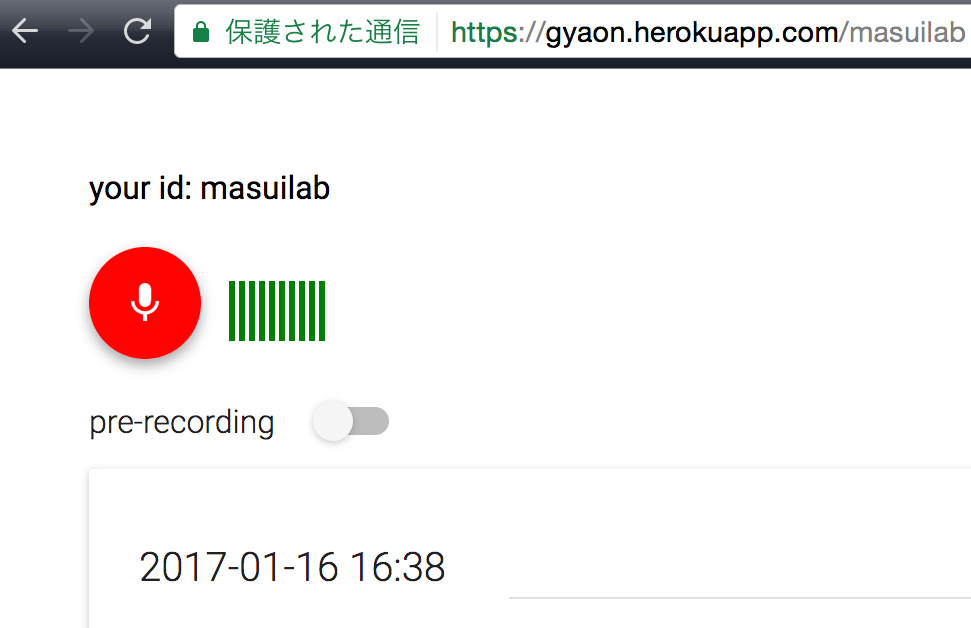
\includegraphics[width=9cm]{images/button.png}}
\caption{録音ボタン}
\label{button}
\end{figure}

\begin{figure}[H]
\centering
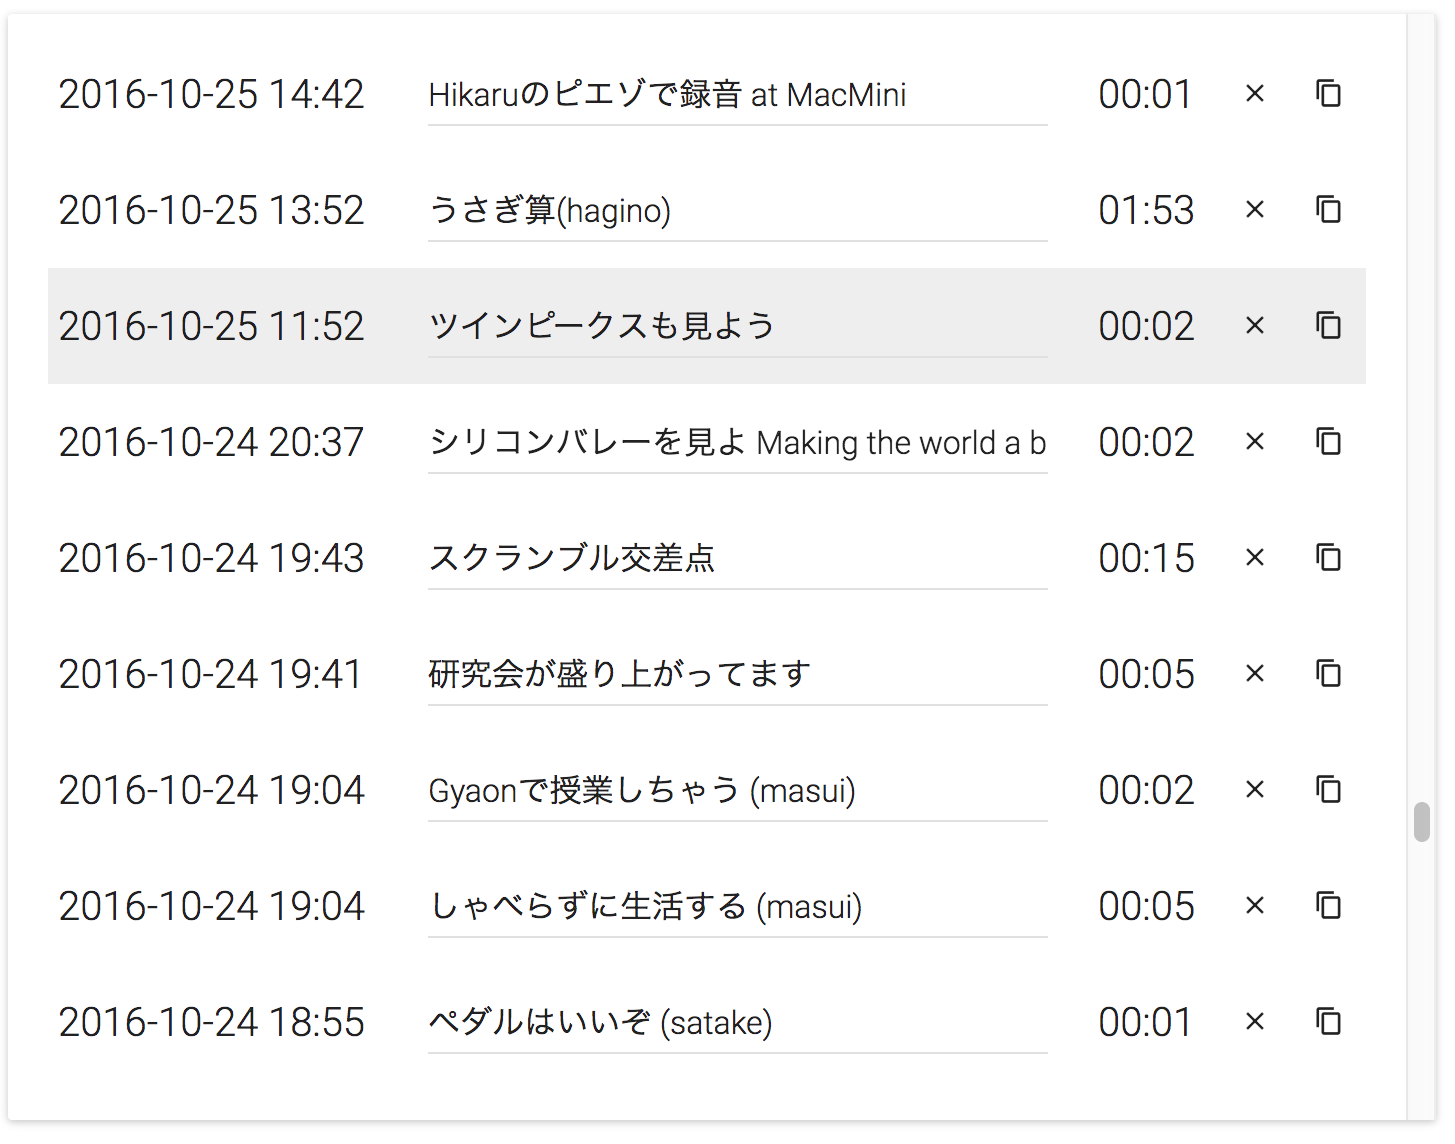
\includegraphics[width=9cm]{images/list.png}
\caption{音声リスト}
\label{list}
\end{figure}

\subsubsection{コメントの追加}
音声リスト内にコメント入力欄があり,クリックすると入力モードに移行する.
音声の内容などを自由に記録することができる.

\subsubsection{音声URLの取得}
音声リストの右側のコピーボタンをクリックすることで,
PCのクリップボードに音声データのURLがコピーされる.
そのままアクセスすれば音声をダウンロードでき,ローカル環境のアプリケーションなどで利用できるほか,
URLを経由して他人に音声を渡すことも可能である.
またNota.inc\footnote{\textsf{http://www.notainc.com/ja/}}のWikiシステム
「Scrapbox」\footnote{\textsf{https://scrapbox.io/}}ではオーディオ記法を利用でき,
決められた書式で音声のURLを入力すると,Gyaonの音声リストと同様にマウスカーソルによる再生が可能となる.

\begin{figure}[H]
\centering
\fbox{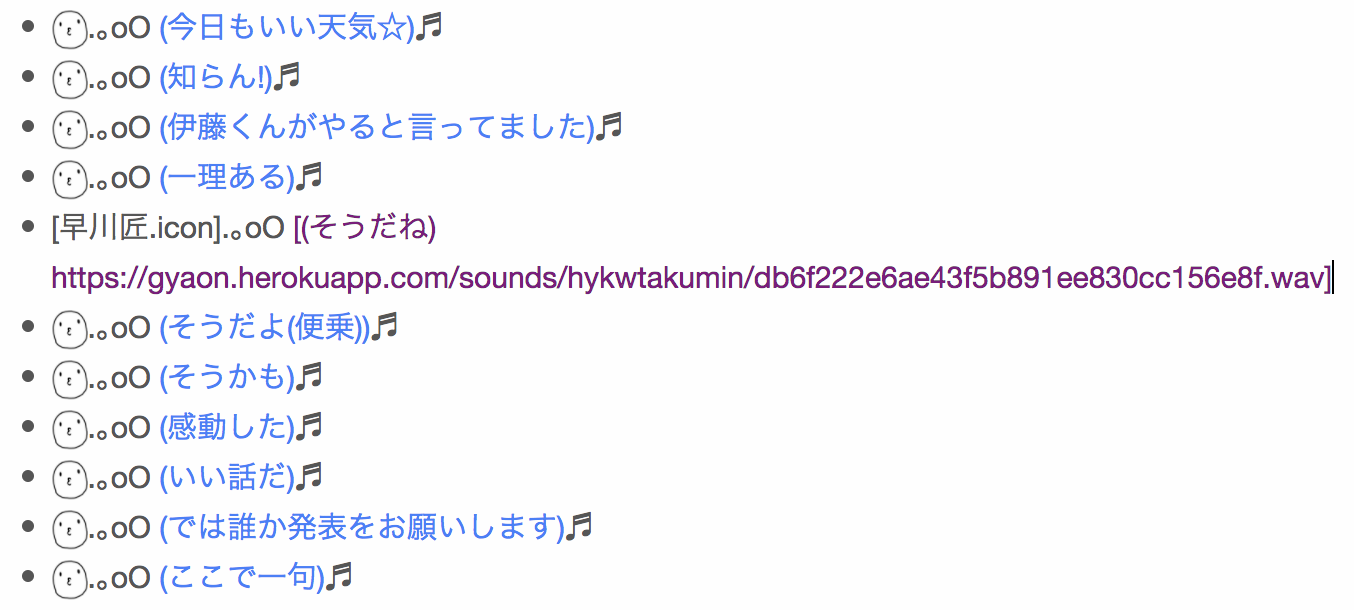
\includegraphics[width=9cm]{images/scrapbox.png}}
\caption{Scrapboxのオーディオ記法}
\label{scrapbox}
\end{figure}

\subsubsection{プリレコーディング機能}
図\ref{button}の「pre-recording」スイッチをONにするとアプリ起動中は常時録音し,
録音ボタンを押す10秒前から音声を記録できる.
もし突然録りたい音が聞こえてきた場合でも逃さず録音することが可能である.
%今いいこと言った!を逃さない
%急に面白い音が聞こえてきても逃さない

\subsubsection{地図機能}
音声データに紐付けられた位置情報をもとに,音声を地図上にマッピングして一覧できる
\footnote{\textsf{地図機能はhttps://gyaon.herokuapp.com/map/にて試験運用中}}.
音声の録音場所が分かることから,その場所の雰囲気や,
景色がいい/この店は美味しいといったその場所ならではの有用な情報を記録/共有できる.

\begin{figure}[H]
\centering
\fbox{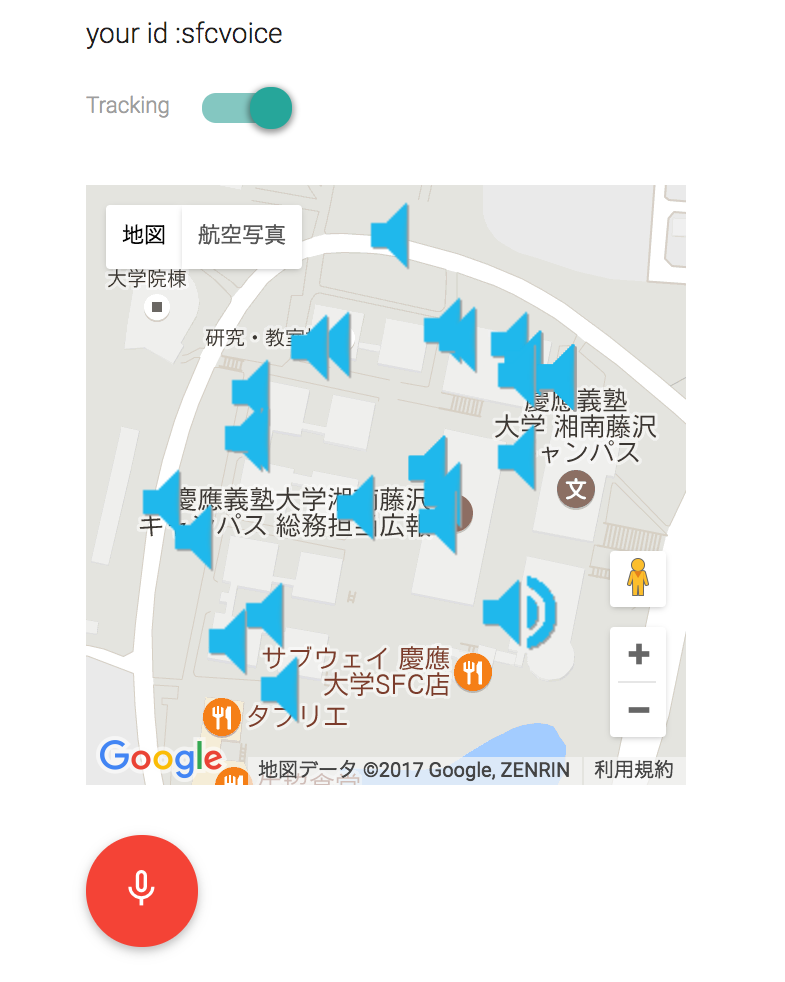
\includegraphics[width=9cm]{images/map.png}}
\caption{地図機能}
\label{map}
\end{figure}

\subsubsection{IDの共有}
GyaonではIDごとに音声を管理しており,
URL末尾でユーザIDを指定できる.
このIDを複数人で共有することでGyaonを共有タスクリストのように利用したり,
ボイスメッセンジャーのような使い方が可能である.

\begin{itembox}[l]
{ユーザIDの指定}
https://gyaon.herokuapp.com/\{ユーザID\}
\end{itembox}

\subsubsection{Gyaonキー}
Gyaonキーアプリケーション\footnote{\textsf{Mac用アプリケーションをhttps://github.com/stkay/GyaonWithKarabinerにて配布中}}
を利用すれば,PCの任意のキーを録音ボタンに設定できる.
これにより,アプリケーションを起動することなく録音可能である.
Webアプリケーションと同様に長押し録音,自動アップロードが行われる.
%キーボードじゃなくて,他の汎用なボタンでもいいよね

\begin{figure}[H]
\centering
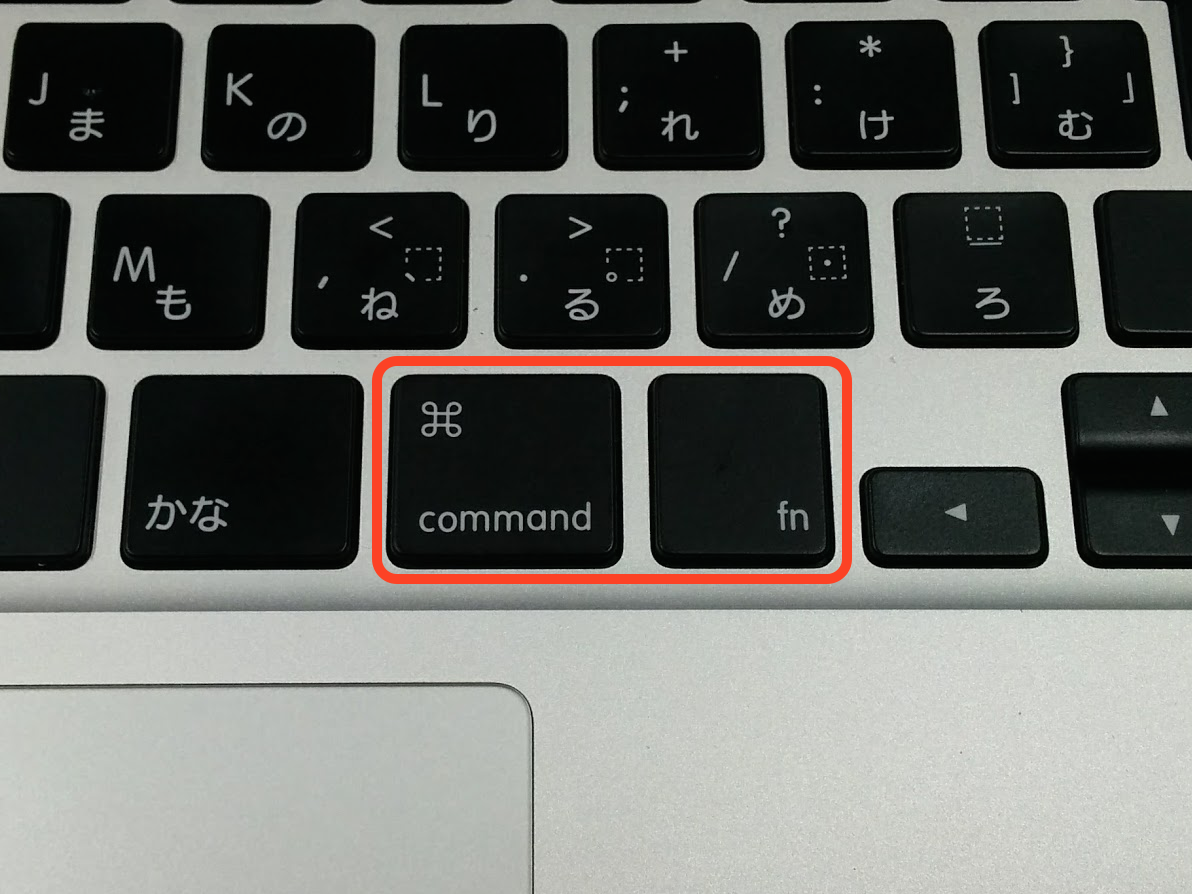
\includegraphics[width=9cm]{images/key.png}
\caption{著者のPCのGyaonキー}
\label{key}
\end{figure}

\subsubsection{Gyaonペダル}
USB接続の汎用なペダル(図\ref{pedal})を接続すれば,楽器演奏/運転中/料理中といった手を使えないシーンでも
ハンズフリー録音が可能となる.
また,ペダルとマイクを接続したRaspberry Pi等を複数用意し,録音専用コンピュータとしてセットアップすることで,
ユビキタスな録音環境を自宅や研究室等に構築可能である.

%冷蔵庫の前に置いて在庫管理,買い物メモ
%トイレ
%キーボードが使えないけどよくいる場所

\begin{figure}[H]
\centering
\fbox{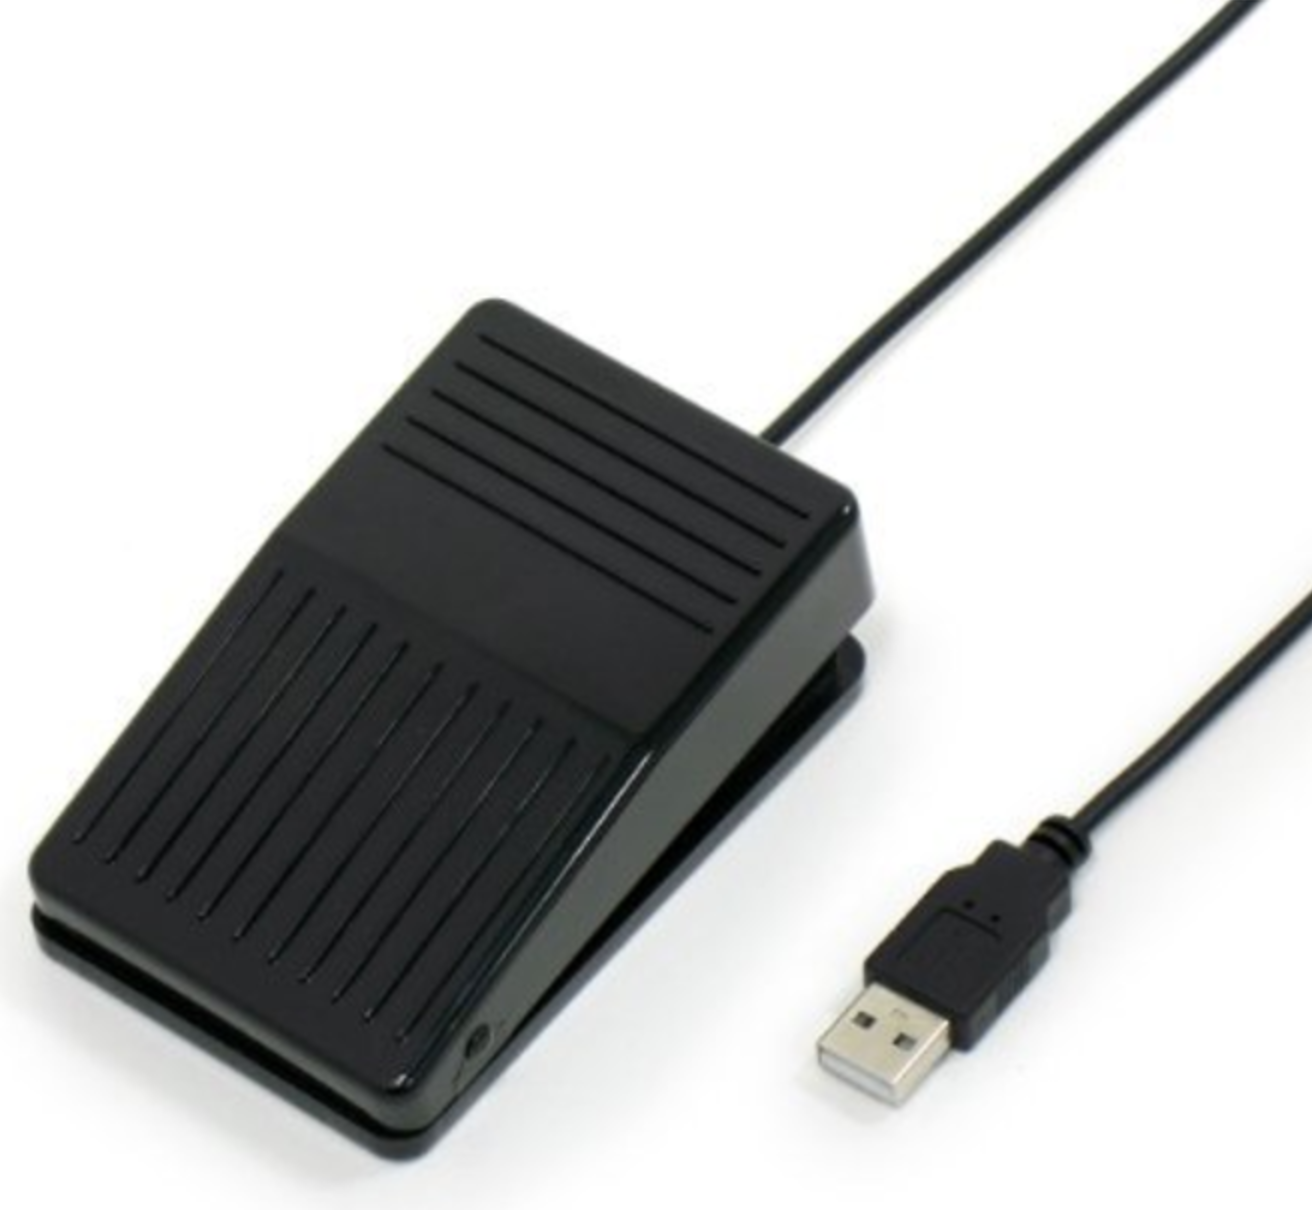
\includegraphics[width=9cm]{images/pedal.png}}
\caption{ペダルの例}
\label{pedal}
\end{figure}

%楽器弾きながらペダル踏んでる画像があるといいかも

\subsection{Android版}

\subsubsection{基本操作}
Android用Gyaonアプリケーションは録音のみ可能で,PC版と同様に長押し録音/自動アップロードが利用できる.(図\ref{app}).
「Your ID」には任意のユーザIDを入力する.
PC版で使用しているユーザIDを入力すれば,スマートフォンでの録音をPCでも聞けるようになる.

\subsubsection{録音ボタンを常駐させる}
図\ref{app}の「STARTSERVICE」ボタンを押すと,録音ボタンをスマートフォン上に常駐させることができる(図\ref{home}).

\subsubsection{利用シーン}
スマートフォンを持ち運べる環境ならいつでもどこでも録音可能である.
外出先で思いついたことを記録したり,
鳥のさえずり/川のせせらぎといった環境音や,アナウンス/街頭演説といった情報を共有する用途にも活用できる.

\begin{figure}[H]
\centering
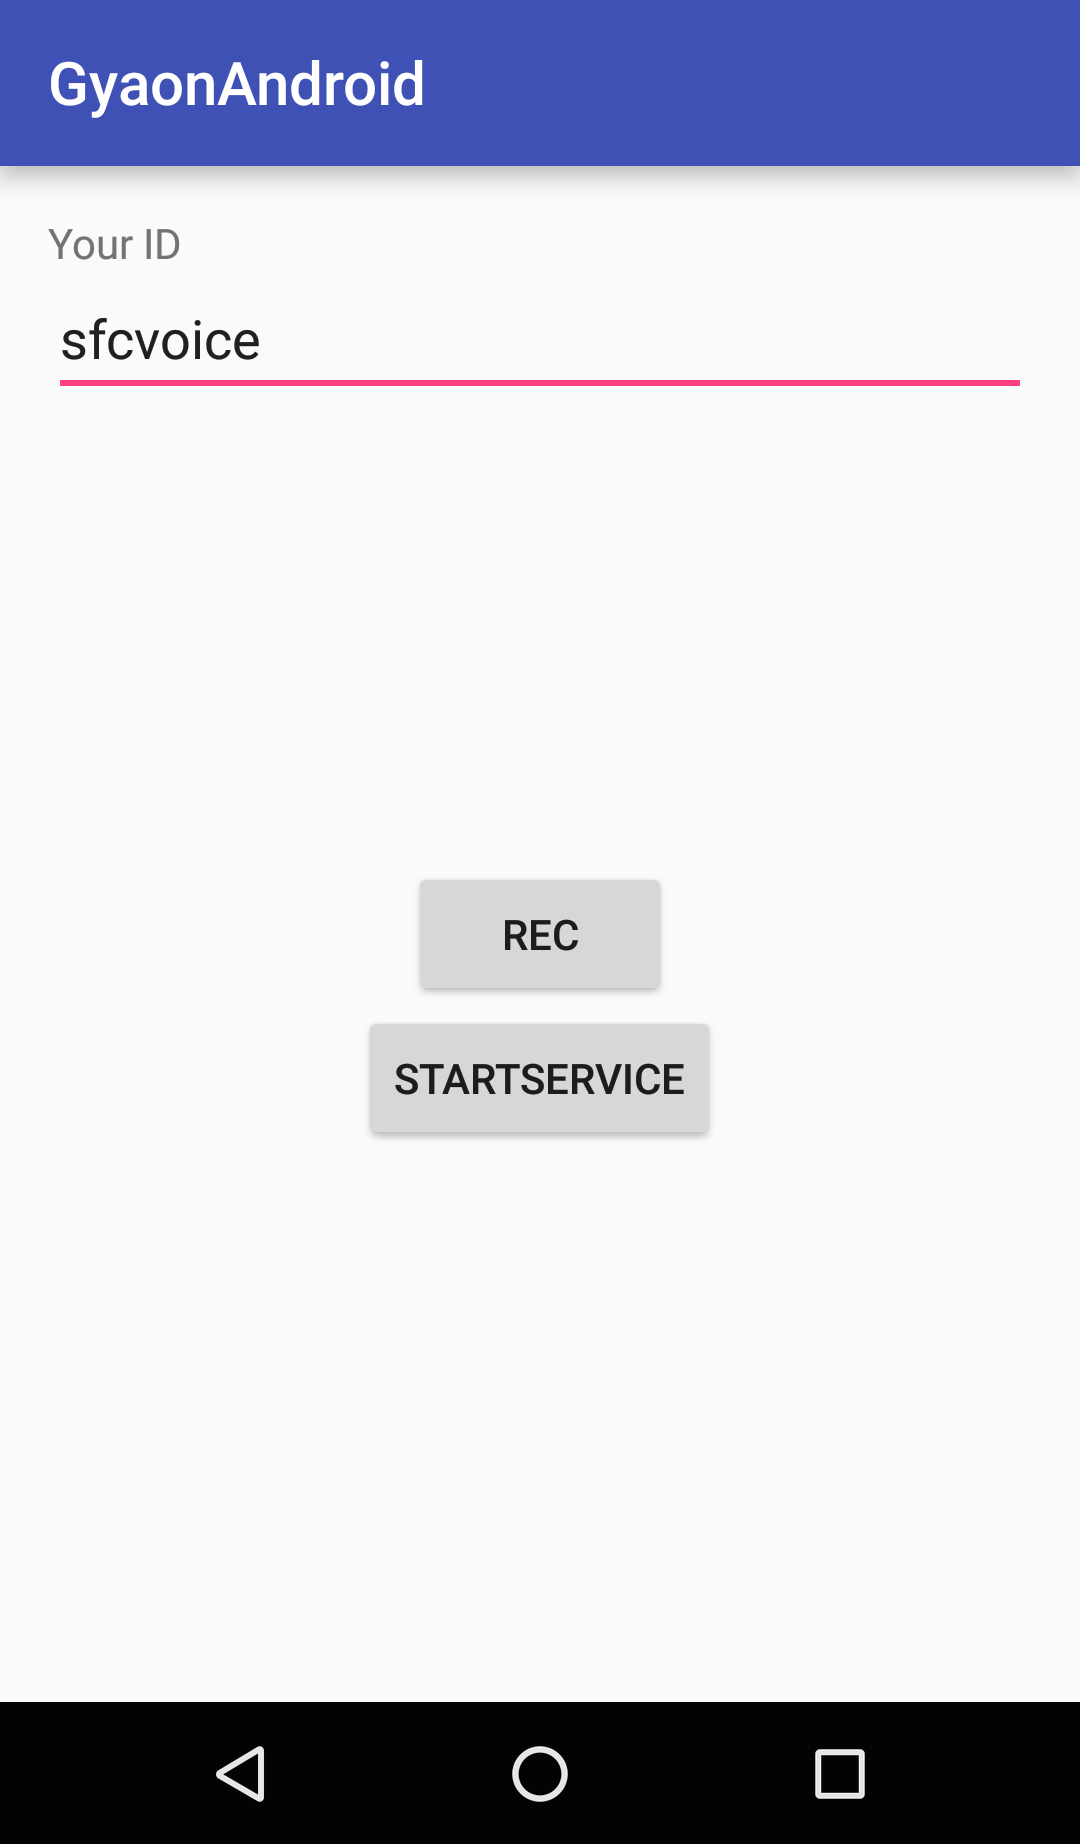
\includegraphics[width=6cm]{images/app.png}
\caption{アプリケーションの起動画面}
\label{app}
\end{figure}

\begin{figure}[H]
\centering
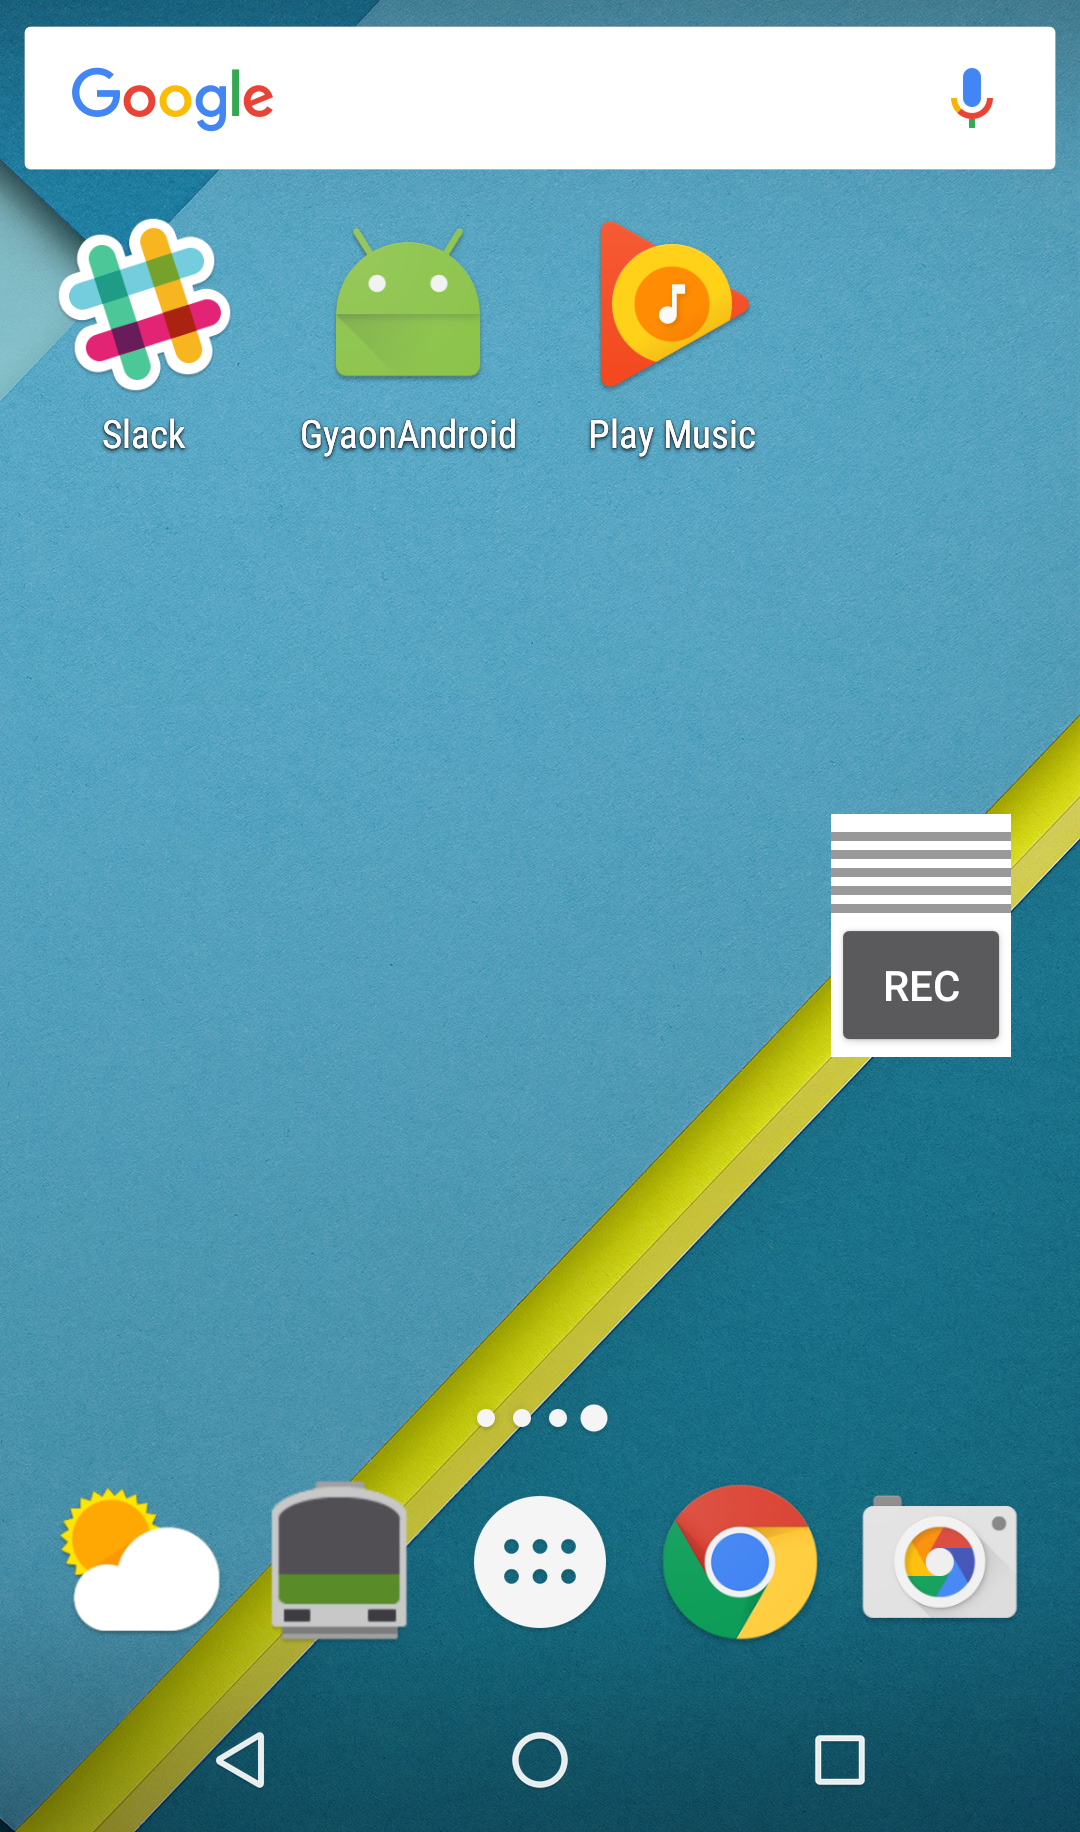
\includegraphics[width=6cm]{images/home.png}
\caption{録音ボタンが配置されたAndroidのホーム画面}
\label{home}
\end{figure}
\chapter{実装}
\label{chap:implementation}

本章では,第2章で述べたシステムの設計を受け,「Gyaon」の実装について述べる.

\newpage

\section{システム構成}

\section{サーバ}

\section{PC版}

\section{Android版}

\section{その他}

\chapter{先行事例}
\label{chap:previous}

本章では,音声利用に関する先行事例を概観する.

\newpage

\section{雰囲気の記録}

日常的な体験や雰囲気を記録するための録音デバイスについて研究が行われている\cite{Poupyrev}.
録音は何かを記録,説明したり,思い出すのに重要な手段だが,日常的に行っている人は少ないと指摘されている.
より気軽に録音できるよう日用品にセンサーを埋め込み,状況の変化に応じて録音/再生するデバイスが提案されている.
日用品に溶け込み,単純明快な録音/再生インターフェースが実現されているが,
本を閉じる/開くといった二値的な状況変化でしか操作できないため,
デバイス単体で複数の音声を管理することが困難になっている.

\section{長時間音声データの管理}

長時間にわたる音声データでは,聞き返したい箇所を効率良く見つけることが困難となる.
この課題に対して,音声データのブラウジングやタグ付けの手法について研究が行われている.

\subsection{ブラウジング}

人間生活に関わる情報を長期間にわたり記録するライフログ関連研究では,
そのログの一部として音声データがよく利用されている\cite{Bell}.
音声データの特徴量を計算し,閾値処理するインターフェースを提供することで再生区間を決定する手法\cite{Kawamura}や,
講義ノートといった手書きメモに対して音声データを関連付ける手法\cite{Stifelman}などが提案されている.

\subsection{タグ付け}

研究ノートの補助的な記録手段として音声データを利用するシステムが提案されている\cite{Kawanishi}.
事前に用意された研究ノートから形態素解析などを利用してキーワードを抽出し,音声データに付与する手法がとられている.

また,音声データの特定のタイミングにタグを付与できる録音システムが開発されている\cite{Fujisaka}.
学生がノートテイキングの補助として使うことを想定しており,重要な説明等を逃さないよう素早くタグ付けが行えるインターフェースが実装されている.

\section{音声ログの検索手法}

音声認識技術を活用したテキストによる音声検索手法が提案されている\cite{Vemuri}.
試作されたアプリケーションでは音声データに含まれる単語からキーワード検索が可能となっているほか,
音声認識の信頼度を文字色に反映させたり,ストップワードを見えにくくするなどして
ユーザが録音の要点を思い出しやすくなるよう配慮されている.

\section{写真との組み合わせ}
写真と音声を組み合わせによる体験記録手法が提案されている\cite{Nakakura}.
写真と手書きだけでは表現できない雰囲気を音声に記録し,
写真によって音声データに一覧性を持たせる仕組みである.
写真が音声の内容把握を助け,音声データの価値を高めることも確認されている.

また,同様の手法によって撮影された写真を,音声とともに閲覧できるWebサイトが公開されている\cite{Masui}.


\chapter{考察}
\label{chap:discussion}

本章では,Gyaonについての考察を行う.

\newpage

\section{単純な録音操作による音声活用の促進}
Gyaonでは録音ボタンを押している間録音し,停止後直ちに音声のアップロードが開始される手順となっており,単純な録音操作を実現している.
著者は開発時から継続的にGyaonを使用しており,単純な録音操作によって,録音行為に対する心理的障壁が低くなったと感じている.
このことから,以前まで手書きやキーボード入力していたメモなどを全て録音するようになり,音声を活用する場面が増えた.
その他にも,様々な場面で音声が活用された.

\paragraph*{研究会での活用}
著者の所属する増井研究会では様々な素材の叩打音を分析する研究が行われており,サンプリングのためにGyaonが活用された.
音声をすぐに確認でき,コメントを付けられる点が好評であった.

また大学が主催する研究発表イベントではリアルタイムな情報共有に活用された.
ブース展示がメインのイベントであったため,面白い展示を見つけた学生がGyaonで共有したり,
楽器のブースでは演奏を録音するなどした.
増井研究会のブースでは常にGyaonを起動していたので,有益な情報を見逃すことなく受け取ることができた.

%共有しやすい
%   URLがあるので「これ聞け」がすぐできる
%
%長時間の音声を録るのはむずい
%   ボタンを押し続けるのは疲れる

%PCもスマホも手元にない時はどうしようもない
%   録音機をばら撒くと解決するかも
%今までのテキストメモに加えて音声メモも管理しないといけない
%   1か所に情報を溜めたいという欲求がある

\paragraph*{雰囲気記録システムとしての活用}
スマートフォンでも簡単に録音できることから,その場の雰囲気を記録する用途に活用された.
鳥のさえずりや川のせせらぎといった環境音を記録して自宅で聞いたり,研究会のミーティングを録音し,
それを振り返りながらメンバーと懐かしむような場面もあった.

\paragraph*{楽器練習支援システムとしての活用}
Gyaonペダルとプレビュー再生機能の組み合わせによって,楽器練習支援システムとして便利に活用できた.
楽器演奏において自分の演奏を客観的に評価することは難しいが,録音を行うことによって解決される.
Gyaonペダルを利用すれば演奏中でも録音でき,録音後のプレビュー再生で演奏をすぐに確認することができる.
演奏/録音/確認を素早く行えることから,従来の録音システムでは実現できなかった新しい練習形態を生み出したといえる.

%さっき撮った音をもう一度聞きたくなった時は大変
%   楽器を持っていて手が空いてない前提
%   画面がなくても操作できれば良い?


\section{外部システムでの音声活用の促進}
Gyaonは音声をアップロードし,URLによって音声データを簡単に取得できるため,Gyaon以外のシステムでも音声活用が促進された.
%URLだけでいいからWebと親和性が高い

\paragraph*{DTMソフトでの活用}
PC上で音楽制作を行うDTMソフトには,録音したり,取り込んだ外部音声ファイルを1つの楽器として利用する
サンプラー機能が存在する.
Gyaonで録音した様々な音声をダウンロードしてDTMソフトに取り込み,作曲に利用することができた.

\paragraph*{「Scrapbox」での活用}
Scrapboxでは音声を文章に埋め込むオーディオ記法が積極的に活用された.
音声の指定にはURLを利用するためGyaonとの親和性が高く,以下のような活用例が見受けられた.

\begin{enumerate}

\item 発表資料を作る

増井研究会ではミーティングで使用する発表資料をScrapboxで作成している.
文章や画像といった資料に加え,予め録音した発表原稿もページに埋め込むことで,
発表者が喋らなくてもプレゼンテーションを行えるようになった.

\item 音声素材をまとめる

積極的に自分の声を録音する研究会メンバーがおり,図\ref{hayakawa}のような音声素材ページが作成された.
ミーティング中に再生して笑いを誘ったり,簡易的な合成音声として活用された.

\begin{figure}[H]
\centering
\fbox{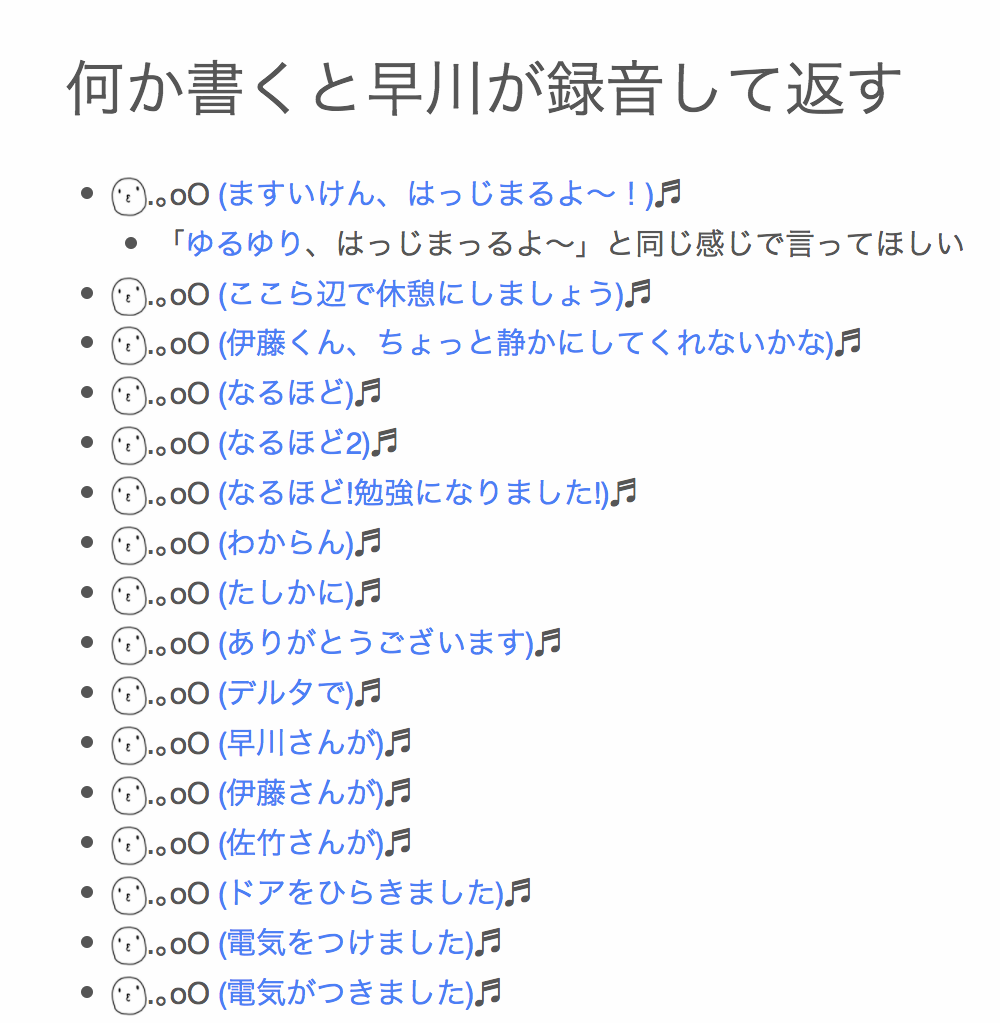
\includegraphics[width=9cm]{images/hayakawa.png}}
\caption{音声素材ページ}
\label{hayakawa}
\end{figure}

\item 単語帳を作る

発音が難しい英単語等をまとめ,その音声を埋め込んだ図\ref{word}のような単語帳が作られた.
マウスカーソルを単語に重ねるだけで発音を確認できるので,より印象に残るものとなった.

\begin{figure}[H]
\centering
\fbox{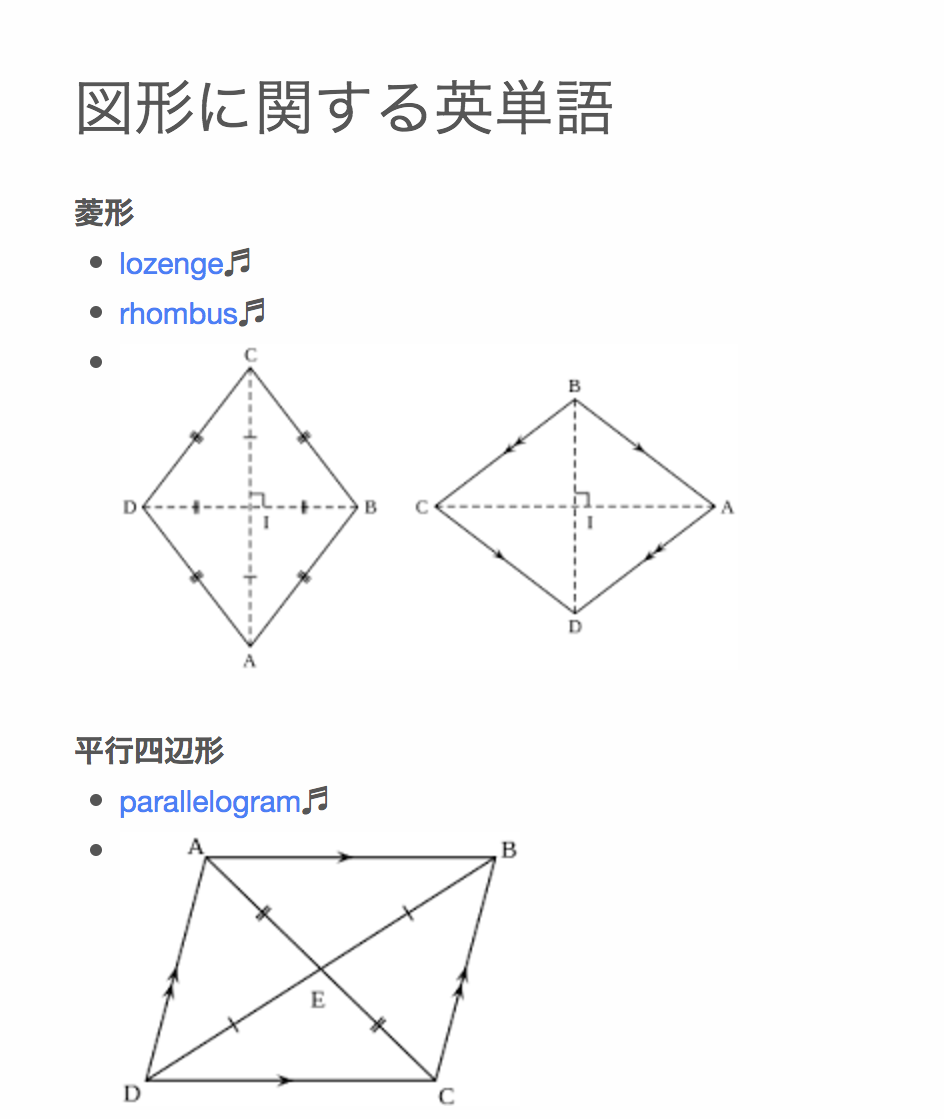
\includegraphics[width=9cm]{images/word.png}}
\caption{音声つき単語帳}
\label{word}
\end{figure}

\end{enumerate}

\section{プライバシー問題}
簡単に録音できるため他者に対するプライバシー侵害の可能性があり,
社会で導入されることに対する心理的障壁は非常に高いと考えられる\cite{Kawamura}.

また,現在のGyaonシステムでは全ての音声が公開されており,誰でもアクセス可能である.
正式なサービスとして運用する場合は,アカウント管理や閲覧権限の設定といった対策が必要である.

\begin{acknowledgment}

本論文の執筆において,担当教員である増井俊之教授に多大なるご指導と貢献をしていただきました.
また,本システムの実装において,研究会OBの橋本 翔氏,桜井雄介氏に多くの貢献と助言を頂きました.
環境情報学部の早川 匠氏には有用な音声素材を提供していただきました.
この場を借りて感謝の意を表します.

\end{acknowledgment}
  % 謝辞。要独自コマンド、include先参照のこと

\begin{bib}[100]
% BibTeXを使う場合
\bibliography{main}

%\begin{thebibliography}{#1}
%
%  \bibitem{参照用名称}
%    著者名:
%    \newblock 文献名,
%    \newblock 書誌情報,出版年.
%
% \bibitem{hoge09}
%   ほげ山太郎,ほげ山次郎:
%   \newblock ほげほげ理論のHCI分野への応用,
%   \newblock ほげほげ学会論文誌,Vol.31,No.3,pp.194-201,2009.
%
% \bibitem{hoge08}
%   Taro Hogeyama, Jiro Hogeyama:
%   \newblock The Theory of Hoge,
%   \newblock {\it The Proceedings of The Hoge Society}, 2008.
%
%\end{thebibliography}

\end{bib}
  % 参考文献。要独自コマンド、include先参照のこと
\appendix
%\chapter{付録の例}

付録を無理矢理出力させるため、てきとうなことを書く。

\section{ほげ}

コマンドは本文と一緒。

\subsection{ふー}

本文と一緒。

\section{ほげほげ}

本文と一緒。

\subsection{ふーふー}

本文と一緒。
    % 付録

\end{document}
